\section{La théorie}
\label{sec:Ch1}

%%%%%%%%%%%%%%%%%%%%%%%%%%%%%%%%%%%% SUBSECTION 1
\subsection{\textbf{Regresion de Breukels : théorie 2D}} 
\label{sec:Ch1.1}

exemple equation
\begin{center}
    \begin{equation}
        C_L = \lambda_5  \alpha^3 +\lambda_6  \alpha^2 + \lambda_7  \alpha + \lambda_8
        \label{eq:Cl_breukels}
    \end{equation}
\end{center}


bla bla 

\begin{figure}[H]
    \centering
    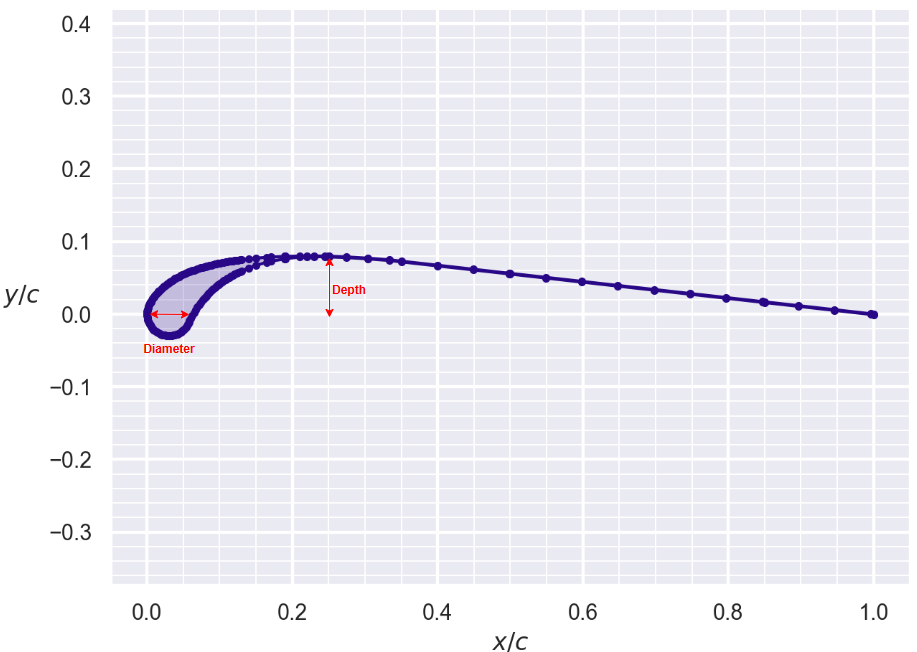
\includegraphics[width=0.5\textwidth]{Pics/01 - Example/airfoil.png}  
    \caption{Profil central d'une SK50-VG avec identification du diamètre et de la cambrure tel que utilisés par la VSM.}
    \label{fig:airfoil}
\end{figure}

%%%%%%%%%%%%%%%%%%%%%%%%%%%%%%%%%%%% SUBSECTION 2
\subsection{\textbf{Regresion de Breukels : théorie 3D}} 
\label{sec:Ch1.2}